% All content is copyright 2023, 2024 the authors.

% To-Do
% -----
% - Hogg asks, can we mention field-level inference in the abstract?


\documentclass[modern]{aastex631}
\usepackage[utf8]{inputenc}
\usepackage{amsmath}
\usepackage{xspace}
\usepackage{graphicx}
\usepackage{bm}
\usepackage{comment}

\setlength{\parindent}{3.5ex}
\sloppy\sloppypar\raggedbottom\frenchspacing

% commands
\newcommand{\abby}[1]{\textbf{Abby says: #1}}
\newcommand{\choice}[1]{\textcolor{teal}{#1}}
\newcommand{\ksf}[1]{\textcolor{purple}{KSF says: #1}}
\newcommand{\catwise}{\textsl{CatWISE}\xspace}
\newcommand{\catwisetwentytwenty}{\textsl{CatWISE2020}\xspace}
\newcommand{\quaia}{\textsl{Quaia}\xspace}
\newcommand{\gaia}{\textsl{Gaia}\xspace}
\newcommand{\wise}{\textsl{WISE}\xspace}
\newcommand{\unwise}{\textsl{unWISE}\xspace}
\newcommand{\vobs}{\boldsymbol{v}_0}
\newcommand{\dd}{\mathrm{d}}
\newcommand{\Cinv}{\boldsymbol{C}^{-1}}
\newcommand{\w}{\mathrm{W}}
\newcommand{\g}{\mathrm{G}}
\newcommand{\npix}{n_\mathrm{pix}}

\begin{document}

\title{Cosmic isotropy and the quasar dipole:\\
Anomalous power on large angular scales}
\author[0000-0001-6069-5383]{Abby E. Williams}
\affiliation{Department of Physics, The University of Chicago, 5640 South Ellis Avenue, Chicago, IL 606137, USA}

\author[0000-0001-8764-7103]{Kate Storey-Fisher}
\affiliation{Donostia International Physics Center, Manuel Lardizabal Ibilbidea, 4, 20018 Donostia, Gipuzkoa, Spain}

\author[0000-0003-2866-9403]{David W. Hogg}
\affiliation{Center for Cosmology and Particle Physics, Department of Physics, New York University, 726 Broadway, New York, NY 10003, USA}
\affiliation{Center for Computational Astrophysics, Flatiron Institute, 162 Fifth Avenue, New York, NY
10010, USA}
\affiliation{Max Planck Institute for Astronomy, K{\"o}nigstuhl 17, 69117 Heidelberg, Germany}

\begin{abstract}\noindent % Hogg insists on this
    There is a discrepancy in amplitude between the dipole measured in the cosmic microwave background and the dipole measured in the distribution of radio and infrared selected quasars.
    These dipoles should be consistent if they are both caused primarily by a local Doppler boost.
    Here we investigate the amplitudes of the large angular-scale spherical harmonic modes ($1\leq\ell\leq 8$) in the sky distribution of two all-sky quasar catalogs, \catwise and \quaia, both of which depend on NASA\! \wise infrared data.
    We adopt a forward-modeling approach to generate all-sky mock density maps for both catalogs and employ a form of simulation-based inference to simultaneously measure the dipole amplitude and the level of any excess power on these large angular scales.
    This inference yields dipole amplitude $X^{+Y}_{-Z}$ in the direction of the kinematic expectation (xx sigma higher than the expected amplitude) and an excess angular power variance amplitude of $X^{+Y}_{-Z}$.
    The excess power we find could indicate a very severe problem with the $\Lambda$CDM model.
    Our view instead is that this power is probably produced by unmodeled selection effects in these two quasar catalogs, and that it is contaminating all quasar dipole measurements that do not account for it.
\end{abstract}

\keywords{foo --- bar}

\section{Introduction}
Our peculiar velocity relative to the rest frame of the Universe creates a dipole in the signals we measure across the sky.
There exists a dipole in the temperature of the CMB, taken to be purely kinematic in origin, which is used to infer a heliocentric velocity of
\begin{equation}
    \label{eq:CMB_velocity}
    v_0 = (369.825\pm 0.070)\,\mathrm{km\, s}^{-1}\ \mathrm{towards}\ (l,b) = (264.021\pm0.009^\circ, 48.253\pm0.004^\circ)
\end{equation}
\citep{planck_collaboration_planck_2020}.
This Doppler boost of the CMB monopole is so well-measured by Planck that its expected modulations and aberrations of the temperature fluctuations have been detected in the CMB spectrum \citep{planck_collaboration_planck_2014}.
\abby{note (emphasize here or somewhere?) that these kinematic effets are strong confirmation that the dipole is caused by our peculiar motion rather than being somehow intrinsic to the CMB!}

The CMB and LSS rest frames should converge under the standard $\Lambda$CDM model; the kinematic dipole anisotropy in the number count of LSS tracers should align with the CMB temperature dipole in direction, with its amplitude modified by a prefactor that depends on the tracer sample.
The predominant approximation comes from \citet{ellis_expected_1984} and gives the expected kinematic dipole from LSS as
\begin{equation}
    \label{eq:ellisbaldwin}
    \vec{\mathcal{D}} \simeq \left[2+x(1+\alpha)\right]\vobs/c
\end{equation}
where $x$ is the number-count slope of the sources at the magnitude limit of the sample and $\alpha$ is the effective spectral index of the sources.

However, there is a growing tension between these two dipole measurements.
Several initial analyses were performed on radio source counts from the 1.4 GHz NRAO VLA Sky Survey (NVSS; \citealt{condon_nrao_1998}).
Though \citet{blake_velocity_2002} found this \textit{matter dipole} to be broadly consistent with the expectation from the CMB, later work such as \citet{singal_large_2011} showed that while the direction of the dipole roughly agreed with the CMB, its amplitude was larger than expected from Eq. \ref{eq:ellisbaldwin}.
Results remain mixed; for example, \citet{darling_universe_2022} found the matter dipole to be consistent with the CMB expectation in both direction and amplitude using radio data from the Very Large Array Sky Survey (VLASS; \citealt{lacy_karl_2020}) and the Rapid
Australian Square Kilometer Array Pathfinder Continuum
Survey (RACS; \citealt{mcconnell_rapid_2020}).

Recently, \citet{secrest_test_2021} (hereafter S21) measured the dipole from a sample of infrared-selected quasars from \catwisetwentytwenty to have more than twice the expected amplitude at $4.9\sigma$ confidence.
\citet{dam_testing_2022} confirmed the S21 result for the identical sample using a different, Bayesian approach.
This suggests that the source of the discrepancy with the CMB dipole is the sample itself (with the specific choices made in its construction) rather than the analysis method.

Several dipole analyses raise systematics as a possible source of the discrepancy ([CITE]).
\abby{do they actually?? at this point I haven't found any major examples, and I think this is part of our point, but to say that no one has raised systematics is a strong claim}
Unmitigated systematics in the source density maps would impact the angular power at several modes, not just $\ell=1$, though investigations of the angular power in these maps at large angular scales ($\ell\lesssim 10$) have been rare.
[but not totally absent: point to papers that investigate this!]

\quaia, a more recent all-sky spectroscopic quasar sample constructed from \gaia and \unwise, offers a new opportunity to measure the LSS dipole \citep{storey-fisher_quaia_2023}.
The catalog is not totally independent from the S21 sample, since both rely on infrared observations from \textit{WISE}—nevertheless, \quaia involves different observations, source selection choices, and systematics modeling, and therefore can serve as a check on the dipole measured in S21.
In this work, we measure the number-count dipole in the S21 and \quaia samples using the approach described in S21 and compare each to their expectation: the direction of the CMB dipole with amplitude given by Eq. \ref{eq:ellisbaldwin}.
However, in order to avoid mode-coupling effects on the measured dipole, we further employ a forward-modeling approach to infer both the amplitude of the dipole in the expected direction and the overall level of excess angular power at multipoles $\ell\le 8$.
\abby{need to explain motivation: why are we doing this? If there is unaccounted-for angular power at other large angular scales, due to mode coupling this could inflate the measured dipole amplitude on the cut sky... (I'm actually not sure how much I trust this statement now since checking out \citet{oayda_cosmic_2024}...)}
We generate mock all-sky quasar density maps with the same selection function as applied to the real data and employ an Approximate Bayesian Computation (ABC) scheme to estimate the parameter posteriors.

% We further measure the angular power at large spherical harmonic modes ($1\leq\ell\leq 8$) in these maps, compare the results to the expected power under $\Lambda$CDM, and explore the robustness of the measured angular power to investigator choices involved in the sample construction and fitting procedure.

This paper is organized as follows.
Section \ref{sec:data} describes the construction of the all-sky samples from \catwise and \quaia.
Section \ref{sec:dipole_expectation} discusses the theoretical matter dipole and the expected amplitude of the dipole in the \catwise and \quaia catalogs under the Ellis-Baldwin approximation.
In Section \ref{sec:AMCSMC} we present our forward-modeling approach and parameter inference via Approximate Bayesian Computation (ABC) using a Sequential Monte Carlo method.
Section \ref{sec:model} explains the all-sky source density model used the generate the mock quasar maps for parameter inference.
Finally, Sections \ref{sec:results} and \ref{sec:discussion} respectively contain the results and subsequent discussion.


\section{The all-sky quasar samples}
\label{sec:data}

Here we describe the construction of two all-sky quasar samples, the \catwise sample used in S21, and the new \quaia sample.

\subsection{The CatWISE2020 Quasar Sample}
\label{sec:catwise}
The S21 quasar sample was constructed from \catwisetwentytwenty, an all-sky infrared catalog constructed from \wise and NEOWISE \citep{marocco_catwise2020_2021}.
The number-count dipole was measured from a final sample of 1,355,352 quasars, shown in Figure \ref{fig:S21_map}.
Here we summarize the steps used in \citet{secrest_test_2021} to construct the sample.

First, to select AGNs, we make a color cut in the initial sources from \catwisetwentytwenty of $\w 1-\w 2\geq0.8$.
The W1 and W2 magnitudes are corrected for galactic reddening using the \citet{planck_collaboration_planck_2014} dust map and extinction coefficients from \citet{wang_optical_2019} (Table 3): total-to-selective extinction ratio $R_V=3.1$, and for the \wise bands, relative extinction ratios $R\w 1=0.039\pm 0.004$ and $R\w 2=0.026\pm 0.004$.
Next, we make the magnitude cut $9\leq\w 1\leq 16.4$. According to S21, beyond $\w 1=16.4$ source density becomes uneven due to \wise's ecliptic scan pattern, and $\w 1=9$ was selected as a lower bound to avoid potential saturation.
To reduce contamination from stars and dust, we make a cut in absolute galactic latitude $\vert b\vert > 30^\circ$.
% This is the fiducial galactic plane cut; see Section \ref{sec:dipole} for an investigation of how other values impact the measured dipole.
To reduce contamination from spurious sources, we also mask several smaller regions: the MCs, bright galaxies from 2MASS, bright artifacts from \wise, and other areas of low completeness.
There are 291 total masked regions.
At this point we convert the list of sources into a healpix map of source densities with $N_\mathrm{side}=64$ \citep{gorski_healpix_2005}.
Note that if any sources in a healpixel are masked, the entire healpixel gets masked.
Finally, S21 noticed a mild inverse linear trend in source density with absolute ecliptic latitude.
Assuming that there is no true correlation between source density and ecliptic latitude (i.e. that the observed trend is a residual systematic), they fit a slope to the absolute sine of ecliptic latitude and correct the source counts by this slope.
We perform this last step when replicating S21's dipole measurement.
However, unless otherwise stated, in other analyses we forego the ecliptic latitude density correction and instead correct the source counts using a selection function map (see Section \ref{sec:selfuncs}).

\begin{figure}
    \centering
    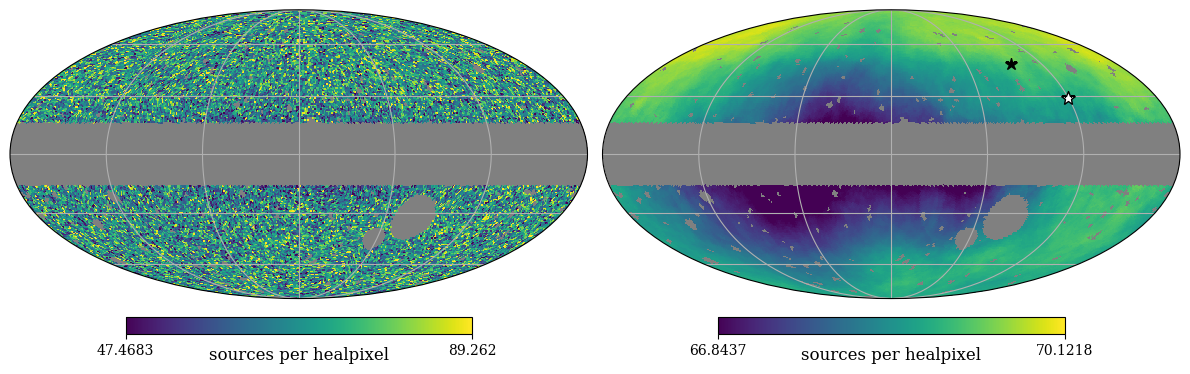
\includegraphics[width=\textwidth]{images/S21_map.png}
    \caption{Healpix density maps ($N_\mathrm{side}=64$) of the S21 sample with the lowest plane cut investigated, $|b|>15^\circ$, in galactic coordinates using a Mollweide projection. The color bar spans the monopole $\pm$ twice the standard deviation of each map. \textit{Left:} Source counts in each healpixel. \textit{Right:} Source counts smoothed to 1 steradian, with the color bar centered at the monopole. The black star marks the direction of the CMB dipole, and the white star marks the direction of the dipole measured in the \textit{fiducial} sample ($|b|>30^\circ$).
    Note the underdensity in source density near the galactic center. \abby{update this plot: add graticule labels, make white star the fiducial S21 result (i.e. no regularization / hp.fit\_dipole() output)}
    \abby{we're doing a $15^\circ$ plane cut in this plot but showing the $30^\circ$ dipole result. I think we should either show only the $30^\circ$ cut or commit to showing the full sky}}
    \label{fig:S21_map}
\end{figure}


\subsection{The Quaia Quasar Sample}
\label{sec:quaia}
The \gaia-\unwise Quasar Catalog, or \quaia, is an all-sky spectroscopic catalog constructed from quasar candidates in \gaia DR3 and infrared observations from \wise \citep{storey-fisher_quaia_2023}.
It spans the largest comoving volume of any existing quasar catalog \abby{is this still true?}, making it especially suited for large-scale precision cosmological measurements.
We use the $G\leq 20.0$ catalog as our fiducial sample, which has 530,364 sources in the fiducial $|b|<30^\circ$ cut, shown in Figure \ref{fig:quaia_map}.
% We also use the less pure $G\leq 20.5$ sample when exploring dependence on magnitude limit.

The construction of the \quaia sample is largely analogous to the S21 method.
\abby{justification for why we don't (need to) correct the magnitudes for reddening like in S21?}
The masks are identical, but we make magnitude cuts in the optical G band ($\mathrm{G}\leq 20.0$) rather than the infrared W1 band.
We also correct the source counts with \quaia's selection function (see Section \ref{sec:selfuncs}).
Figure \ref{fig:quaia_map} shows the \quaia sample after correcting by the selection function.

\begin{figure}
    \centering
    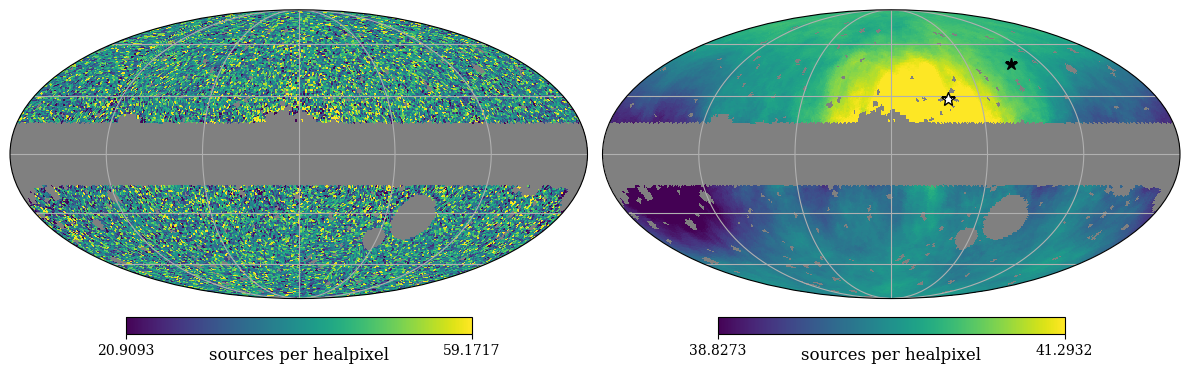
\includegraphics[width=\textwidth]{images/quaia_map.png}
    \caption{Healpix density maps ($N_\mathrm{side}=64$) of the \quaia sample with the lowest plane cut, $|b|>15^\circ$, in galactic coordinates using a Mollweide projection. The source densities have been corrected using the $G<20.0$ selection function map. The masks are identical to those used in the S21 sample (Figure \ref{fig:S21_map}), with the color bar again spanning the monopole $\pm$ twice the standard deviation of each map. \textit{Left:} Source counts in each healpixel. \textit{Right:} Source counts smoothed to 1 steradian. The black star marks the direction of the CMB dipole, and the white star marks the direction of the dipole measured in the \textit{fiducial} sample ($|b|>30^\circ$). Note the unevenness in source density around the galactic plane, in particular the slight overdensity just above the galactic center. There are some extra masked pixels at low galactic latitudes in places with zero quasar counts.}
    \label{fig:quaia_map}
\end{figure}


\subsection{Selection functions}
\label{sec:selfuncs}
For each sample, we generate a selection function, which gives the completeness in each pixel relative to the predicted number of quasars that would be observed in the absence of any selection effects.
To model the selection function, \cite{storey-fisher_quaia_2023} uses a Gaussian process to fit healpix maps ($N_\mathrm{side}=64$; \citealt{gorski_healpix_2005}) of the systematics templates to the source counts in each healpixel.
The systematics templates for \quaia are dust extinction, \gaia and \unwise source density, and those missions' scanning laws.\abby{might want to be more specific ?}
For \catwise, the templates are the \unwise source density... \abby{zodi?}
To correct the observed counts by the selection function, we simply divide the counts by the relative completeness in each pixel.
Figure \ref{fig:selfuncs} shows the selection function maps generated for each quasar sample.

[ Figure: selection functions! ]


\section{The dipole expectation}
\label{sec:dipole_expectation}
Under the kinematic interpretation of the dipole, both the CMB and matter dipole anisotropies are caused by our proper motion with respect to the frame in which the CMB is maximally isotropic.
Therefore the expected direction of the matter dipole is the same as the CMB dipole (Eq. \ref{eq:CMB_velocity}).
The expected amplitude of the matter dipole, however, depends on the velocity $\vobs$ of the observer and the properties of the sources in the sample, in particular the number-count slope $x$ and the effective spectral index $\alpha$ of the sample.
Eq. \ref{eq:ellisbaldwin} is the result of two special relativistic effects: there is an abberration effect causing sources in direction $\hat{v}_0$ to appear closer together, and there is a flux effect causing sources in direction $\hat{v}_0$ to appear brighter.
These effects result in additional dependencies on $x$, the slope of the number of sources at the magnitude limit of the sample, and $\alpha$, the effective spectral index of the sample.
As described in \citet{ellis_expected_1984}, both of these values come in at roughly order unity.

We calculate $x$ using
\begin{equation}
    x \equiv -\left.\frac{\dd\ln N(>S_\nu)}{\dd\ln S_\nu}\right|_{S_\mathrm{min}} ~,
\end{equation}
where $S_\nu$ is the flux density, $N(>S_\nu)$ is the number of sources above a given flux density limit, and $S_\mathrm{min}$ is the flux-density limit of the sample.
The results for both samples are shown in Figure \ref{fig:alphas_xs}.
For \catwise, the number-count slope at the fiducial magnitude limit $\w 1=16.4$ is $x=1.75$.
For \quaia, the number-count slope at the fiducial magnitude limit $\g =20.0$ is $x=1.30$.

To calculate $\alpha$, we assume that the flux density of each source roughly follows a power law, $S_\nu(\nu)\sim\nu^{-\alpha}$.
We can estimate $\alpha$ for any source with flux measurements at two or more frequencies.
If we have magnitudes of the source in two spectral bands, $m_1$ and $m_2$ in the AB system, from the definition of magnitude they are related to flux by
\begin{equation}
    (m_1-m_2)_\mathrm{AB}=-2.5(\log S_{\nu,m_1}-\log S_{\nu,m_2}) ~,
\end{equation}
where $S_{\nu}$ is the flux density (units of W m$^{-2}$ Hz$^{-1}$).
Since magnitudes in the AB system are defined relative to a source with flat spectrum, $\nu S_\nu=$ constant, $\alpha$ can be computed from the slope of the AB magnitudes,
\begin{equation}
    \alpha = -\frac{\dd\log S_\nu}{\dd\log\nu} \approx -\frac{\log S_{\nu,m_1}-\log S_{\nu,m_2}}{\log\left(\nu_{m_1}/\nu_{m_2}\right)} = -\frac{1}{2.5}\frac{(m_1-m_2)_{\mathrm{AB}}}{\log(\lambda_{m_2}/\lambda_{m_1})} ~,
\end{equation}
where $\lambda$ is the wavelength, $\lambda=\frac{c}{\nu}$.
Both \gaia and \wise report magnitudes in the Vega system, so we convert to AB magnitudes using the photometric zeropoints in each band (BP$-$RP and W1$-$W2).
The $\alpha$ distributions for both samples are shown in Figure \ref{fig:alphas_xs}.
Following S21, we choose the effective spectral index to be the mean $\alpha$ of each sample.
For \catwise, this is $\alpha=1.26$, while for \quaia, the mean is $\alpha=0.71$.

From Eq. \ref{eq:ellisbaldwin}, with the velocity inferred from the CMB dipole (Eq. \ref{eq:CMB_velocity}) the expected dipole amplitude in the fiducial S21 sample is $\mathcal{D}_\mathrm{S21}\sim 0.0074$.
For \quaia, the expected dipole amplitude in the fiducial sample is $\mathcal{D}_\mathrm{Quaia}\sim 0.0052$.
\abby{how many sig figs to quote here, given that this in an imprecise measurement? should I even only quote one? I currently use two sig figs for the simulations}
[
The sources included in each sample change as we investigate the effect of parameter choices involved in their construction (Sections \ref{sec:S21_choices} and \ref{sec:quaia_choices}), meaning the $\alpha$ distributions and number-count curves change too.
We checked that this change has minimal impact on the expected dipole amplitude, so we use the fiducial values when comparing the measured amplitudes in each sample.
]
\abby{might fully cut this, I don't think we're including these parameter choice tests anymore}

\subsection{Relationship between $|\vec{\mathcal{D}}|$ and $C_1$}

Existing literature typically describes the sky dipole using one of two conventions.
The dipole anisotropy in the source counts in direction $\hat n$ on the sky can be expressed as
\begin{equation}
    \frac{\delta N}{N}(\hat n) = \vec{\mathcal{D}}\cdot \hat n
\end{equation}
where $\vec{\mathcal{D}}\equiv(\mathcal{D}_x,\mathcal{D}_y,\mathcal{D}_z)$ is a vector whose components are the amplitudes of three orthogonal dipole templates.
This is the convention used in \citet{secrest_test_2021}.
There is a direct transformation between this dipole amplitude $|\vec{\mathcal{D}}|$ and the $\ell=1$ mode of the angular power spectrum $C(\ell)$:

\begin{equation}
    C_1 = \frac{4\pi}{9}|\vec{\mathcal{D}}|^2
\end{equation}
with the specific components related to the spherical harmonic coefficients as
\begin{equation}
    \mathcal{D}_{(x,y,z)} = \sqrt{\frac{3}{4\pi}}\,a_{1(-1,0,1)}
\end{equation}
\abby{Hogg: not sure the best way to write this... \citet{gibelyou_dipoles_2012} aligns the dipole in the positive $z$ direction and then only expresses this relationship in terms of $|\vec{\mathcal{D}}|$ and $a_{10}$, without loss of generality. this is definitely the easiest to write, but it's a bit removed from what we do in practice (we use galactic coordinates and so do have to transform all three dipole components).}

\begin{figure}
    \centering
    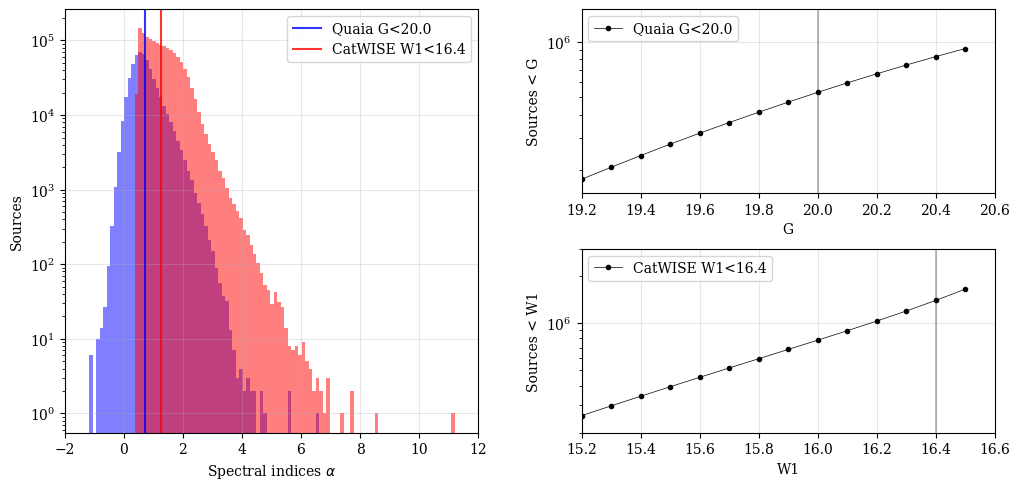
\includegraphics[width=\textwidth]{images/alphas_xs_G20.5.png}
    \caption{The spectral indices $\alpha$ and number-count slopes $x$ used to calculate the expected dipole amplitude for the \quaia and S21 fiducial samples. \textit{Left:} Histogram of the spectral indices $\alpha$ calculated for each source in the \quaia (blue) and S21 (red) fiducial samples. The vertial lines indicate the mean ($\bar\alpha=$0.71 and 1.26, respectively), which is taken as the effective value and used in Eq. \ref{eq:ellisbaldwin}. Note the sharp minimum cutoff in S21 due to the $W1-W2$ color cut made when constructing the sample. \textit{Right:} Number of sources as a function of the magnitude limit in the \quaia (top) and S21 (bottom) samples. The slope of the curve ($x=$1.30 and 1.75, respectively) at the magnitude limit of the fiducial sample, indicated by the grey vertical lines, is the number-count slope used in Eq. \ref{eq:ellisbaldwin}.}
    \label{fig:alphas_xs}
\end{figure}


\section{ABC-SMC}
\label{sec:AMCSMC}

We use a forward-modeling approach to infer the dipole and any excess angular power that may be present in the quasar catalogs.
In particular, we employ Approximate Bayesian Computation (ABC), a likelihood-free parameter inference method, implemented using the \texttt{pyABC} package \citep{schalte_pyabc_2022}.
In particular, \texttt{pyABC} uses a sequential Monte-Carlo (SMC) scheme to iteratively update the posterior probability distribution.
ABC-SMC requires an executable forward-process model and a prior distribution for each parameter.




\section{The all-sky model}
\label{sec:model}

We model the quasar density at some sky position $(\theta,\phi)$ as a stochastic function with two free parameters: the kinematic dipole amplitude $|\vec{\mathcal{D}}_k|$ and the level of excess angular power $\bar C$.
We assume that the kinematic dipole points in the same direction as the CMB dipole, $(\ell,b)=(264^\circ,48^\circ)$, with some amplitude $|\vec{\mathcal{D}}_k|$.
The model also has the freedom to be anisotropic at the largest angular scales, $1\le\ell\le 8$, with excess angular power which is flat in $C(\ell)$ space.
The spherical harmonic coefficients $a_{\ell m}$ are drawn stochastically from a Gaussian whose width depends on $\bar C$.
The model is called on a healpixel grid, and the kinematic dipole map $\mathcal{D}_k(\theta,\phi)$ and excess power map $\gamma(\bar C)(\theta,\phi)$ are constructed in overdensity space, so their average over all pixels is zero.
\abby{how do we feel about $\gamma$ as the excess power map?... not sure I'm a fan but not sure if there is an existing convention for this}

To convert from overdensity to quasar counts, we take
\begin{equation}
    \lambda(\theta,\phi) = (1 + \mathcal{D}_k(\theta,\phi) + \gamma(\bar C)(\theta, \phi)) \cdot \rho
\end{equation}
where $\rho$ is the quasar base rate \abby{need to explain this}, $\mathcal{D}_k(\theta,\phi)$ is the kinematic dipole contribution to the overdensity, and $\gamma(\bar C)(\theta,\phi)$ is the excess angular power contribution to the overdensity at angle $(\theta,\phi)$ on the sky.
Note that the total dipole in the map is the sum of the kinematic dipole and the ``excess power" dipole,
\begin{equation}
    \vec{\mathcal{D}}_\mathrm{tot}=\vec{\mathcal{D}}_k + \vec{\mathcal{D}}_\gamma 
\end{equation}

The map $\lambda(\theta,\phi)$ gives the number of quasars observed in a healpixel centered at $(\theta,\phi)$ in the absence of shot noise and selection effects.
To incorporate these observational effects, we multiply the map by the selection function (Section \ref{sec:selfuncs}) and draw the final quasar counts in each pixel from a Poisson distribution with expectation $\lambda(\theta,\phi)$.

[ Figure (?): example mocks, maybe even extreme cases that don't look like the data (e.g. very low excess power, very high excess power) to give the reader a sense of range]


\section{Results}
\label{sec:results}

We use the ABC-SMC algorithm (Section \ref{sec:AMCSMC}) and the forward-process sky model described in Section \ref{sec:model} to infer both $|\vec{\mathcal{D}}_{\mathrm{proj},k}|$ the amplitude of the quasar dipole projected along the CMB dipole direction, and $\bar C$, the average excess angular power at the largest angular scales, $1\le\ell\le 8$.
We require 500 accepted samples per generation and run for 18 generations.

\begin{figure}
    \centering
    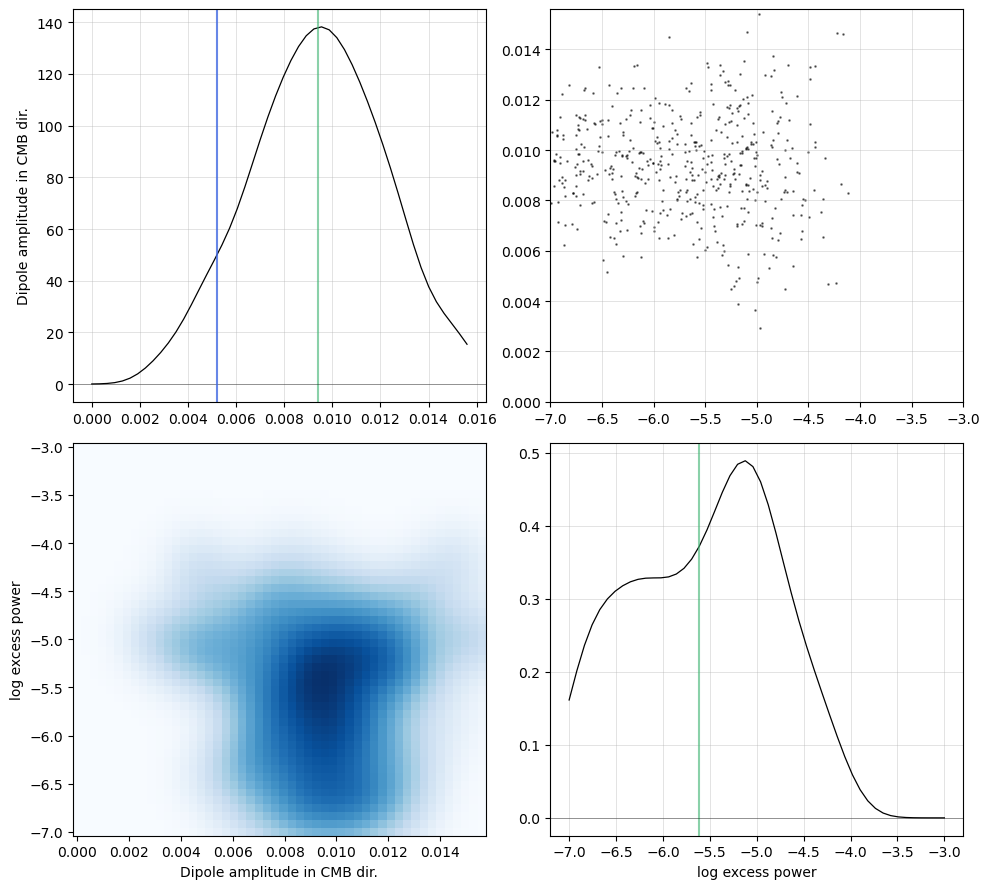
\includegraphics[width=0.9\linewidth]{images/quaia_ABC_posterior.png}
    \caption{Posterior distribution for the \quaia sample. The vertical blue line indicates the expected dipole amplitude from the Ellis-Baldwin test (0.0052), while the vertical green lines indicate the median of the parameters used to generate the accepted samples.}
    \label{fig:quaia_posterior}
\end{figure}

\begin{figure}
    \centering
    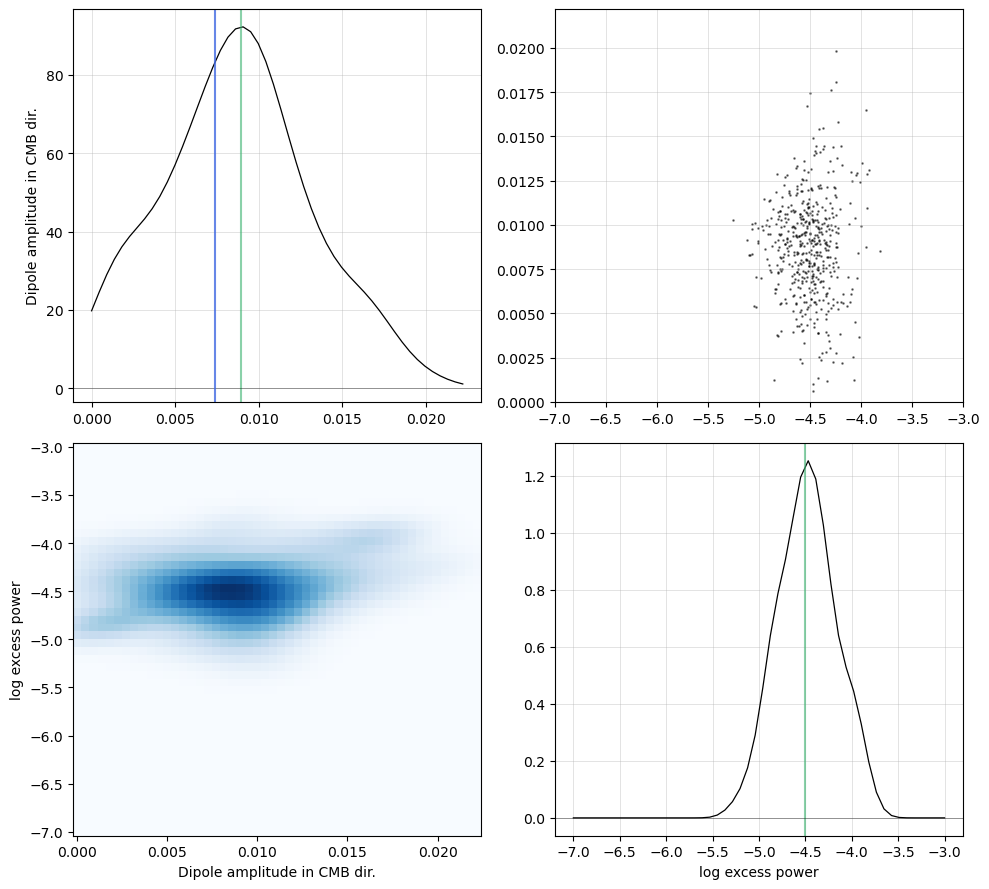
\includegraphics[width=0.9\linewidth]{images/catwise_ABC_posterior.png}
    \caption{Posterior distribution for the \quaia G<20.0 sample. The vertical blue line indicates the expected dipole amplitude from the Ellis-Baldwin test (0.0074), while the vertical green lines indicate the median of the parameters used to generate the accepted samples.}
    \label{fig:catwise_posterior}
\end{figure}

[ Figure (?): Cell results from posteriors vs data ]


\section{Discussion}
\label{sec:discussion}

\appendix{Key points before I forget}
\begin{enumerate}
    \item \textit{this is not a precise measurement!!!}
    \begin{enumerate}
        \item the expected dipole amplitude is an approximation
        \item we know to expect some level of shot noise and cosmological dipole, so we don't even expect the measured dipole in these catalogs to be the kinematic dipole even in the absence of anomalous power (see Cheng et al. paper 2023)
    \end{enumerate}
    \item (connected to above point) we can't make a [robust/principled/accurate/correct] choice of regularization strength since we don't have a noise model. we can see this in our mock results
    \begin{enumerate}
        \item is it possible to have a ``correct'' choice of regularization $\Lambda$? does it depend which $\ell$ we care about? my current understanding is that if there is excess power on multiple angular scales, there is not a single choice of $\Lambda$ that can correctly recover the power at each scale $\ell$ (maybe unless we're in the unique case where the excess power $C(\ell)$ projects onto the sky mask in such a way that a single value of $\Lambda$ correctly accounts for the impact of the non-orthogonalities of the spherical harmonics)
    \end{enumerate}
\end{enumerate}

\bibliography{references}

\end{document}